%%%%%%%%%%%%%%%%%%%%%%%%%%%%%%%%%%%%%%%%%%%%%%%%%%%%%%%%%%%%%%%%%
%_____________ ___    _____  __      __ 
%\____    /   |   \  /  _  \/  \    /  \  Institute of Applied
%  /     /    ~    \/  /_\  \   \/\/   /  Psychology
% /     /\    Y    /    |    \        /   Zuercher Hochschule 
%/_______ \___|_  /\____|__  /\__/\  /    fuer Angewandte Wissen.
%        \/     \/         \/      \/                           
%%%%%%%%%%%%%%%%%%%%%%%%%%%%%%%%%%%%%%%%%%%%%%%%%%%%%%%%%%%%%%%%%
%
% Project     : Seminararbeit
% Title       : 
% File        : einfluss.tex Rev. 00
% Date        : 10.10.2012
% Author      : Till J. Ernst
%
%%%%%%%%%%%%%%%%%%%%%%%%%%%%%%%%%%%%%%%%%%%%%%%%%%%%%%%%%%%%%%%%%
\thispagestyle{empty}
\chapter{Einfluss \textit{Sozialer Medien} auf das \textit{Subjektive Wohlbefinden}}\label{chap.einfluss}
\glsreset{swb}
In diesem Kapitel wird der Einfluss erläutert, wie sich \gls{sm} auf das \gls{swb} auswirken. Dazu werden verschieden Studien untersucht und mittels \gls{cm} grafisch zusammengeführt. Der Einfluss auf das \gls{swb} ist von verschiedenen Faktoren abhängig, welche in \textit{Abbildung~\ref{fig.ConceptMapSwbSm}} ersichtlich sind.\newline
Die Grafik stellt den Zusammenzug unterschiedlicher Studien dar, die sich mit den Auswirkungen von \gls{sm} auf das \gls{swb} auseinander setzen. Darin sind die verschiedenen Konstrukte ersichtlich, die in den Studien verwendet wurden. Gelesen wird die Grafik ausgehend von den \gls{sm} entlang den Verbindungslinien bis hin zum \gls{swb}.\newline
In den folgenden Unterkapiteln werden diese Konzepte anhand der Grafik erläutert. Dazu wird die Grafik in verschiedene Stränge unterteilt, um den komplexen Informationsgehalt in übersichtliche Häppchen aufzuteilen. Die Stränge sollen von den \gls{sm} ausgehend, über wichtige Konzepte und Begriffe, bis hin zum \gls{swb} führen. \newline
In der folgenden Erläuterungen werden die verwendeten Begriffe in ihrer originalen, englischen Form übernommen, damit die ursprüngliche Bedeutung durch eine unsachgemässe Übersetzung nicht verfälscht wird. Bei der jeweiligen Worterklärung wird für die erhöhte Lesbarkeit eine entsprechende deutsche Übersetzung mitgeliefert, wobei hier zu beachten ist, dass die Begriffe in den Studien unterschiedlich verwendet werden und die Bedeutung je nach Verwendung des Autors leicht abweichen können.\newline

%Abbildung von ConceptMap SWB und SM
\begin{figure}[H]
	\centering
		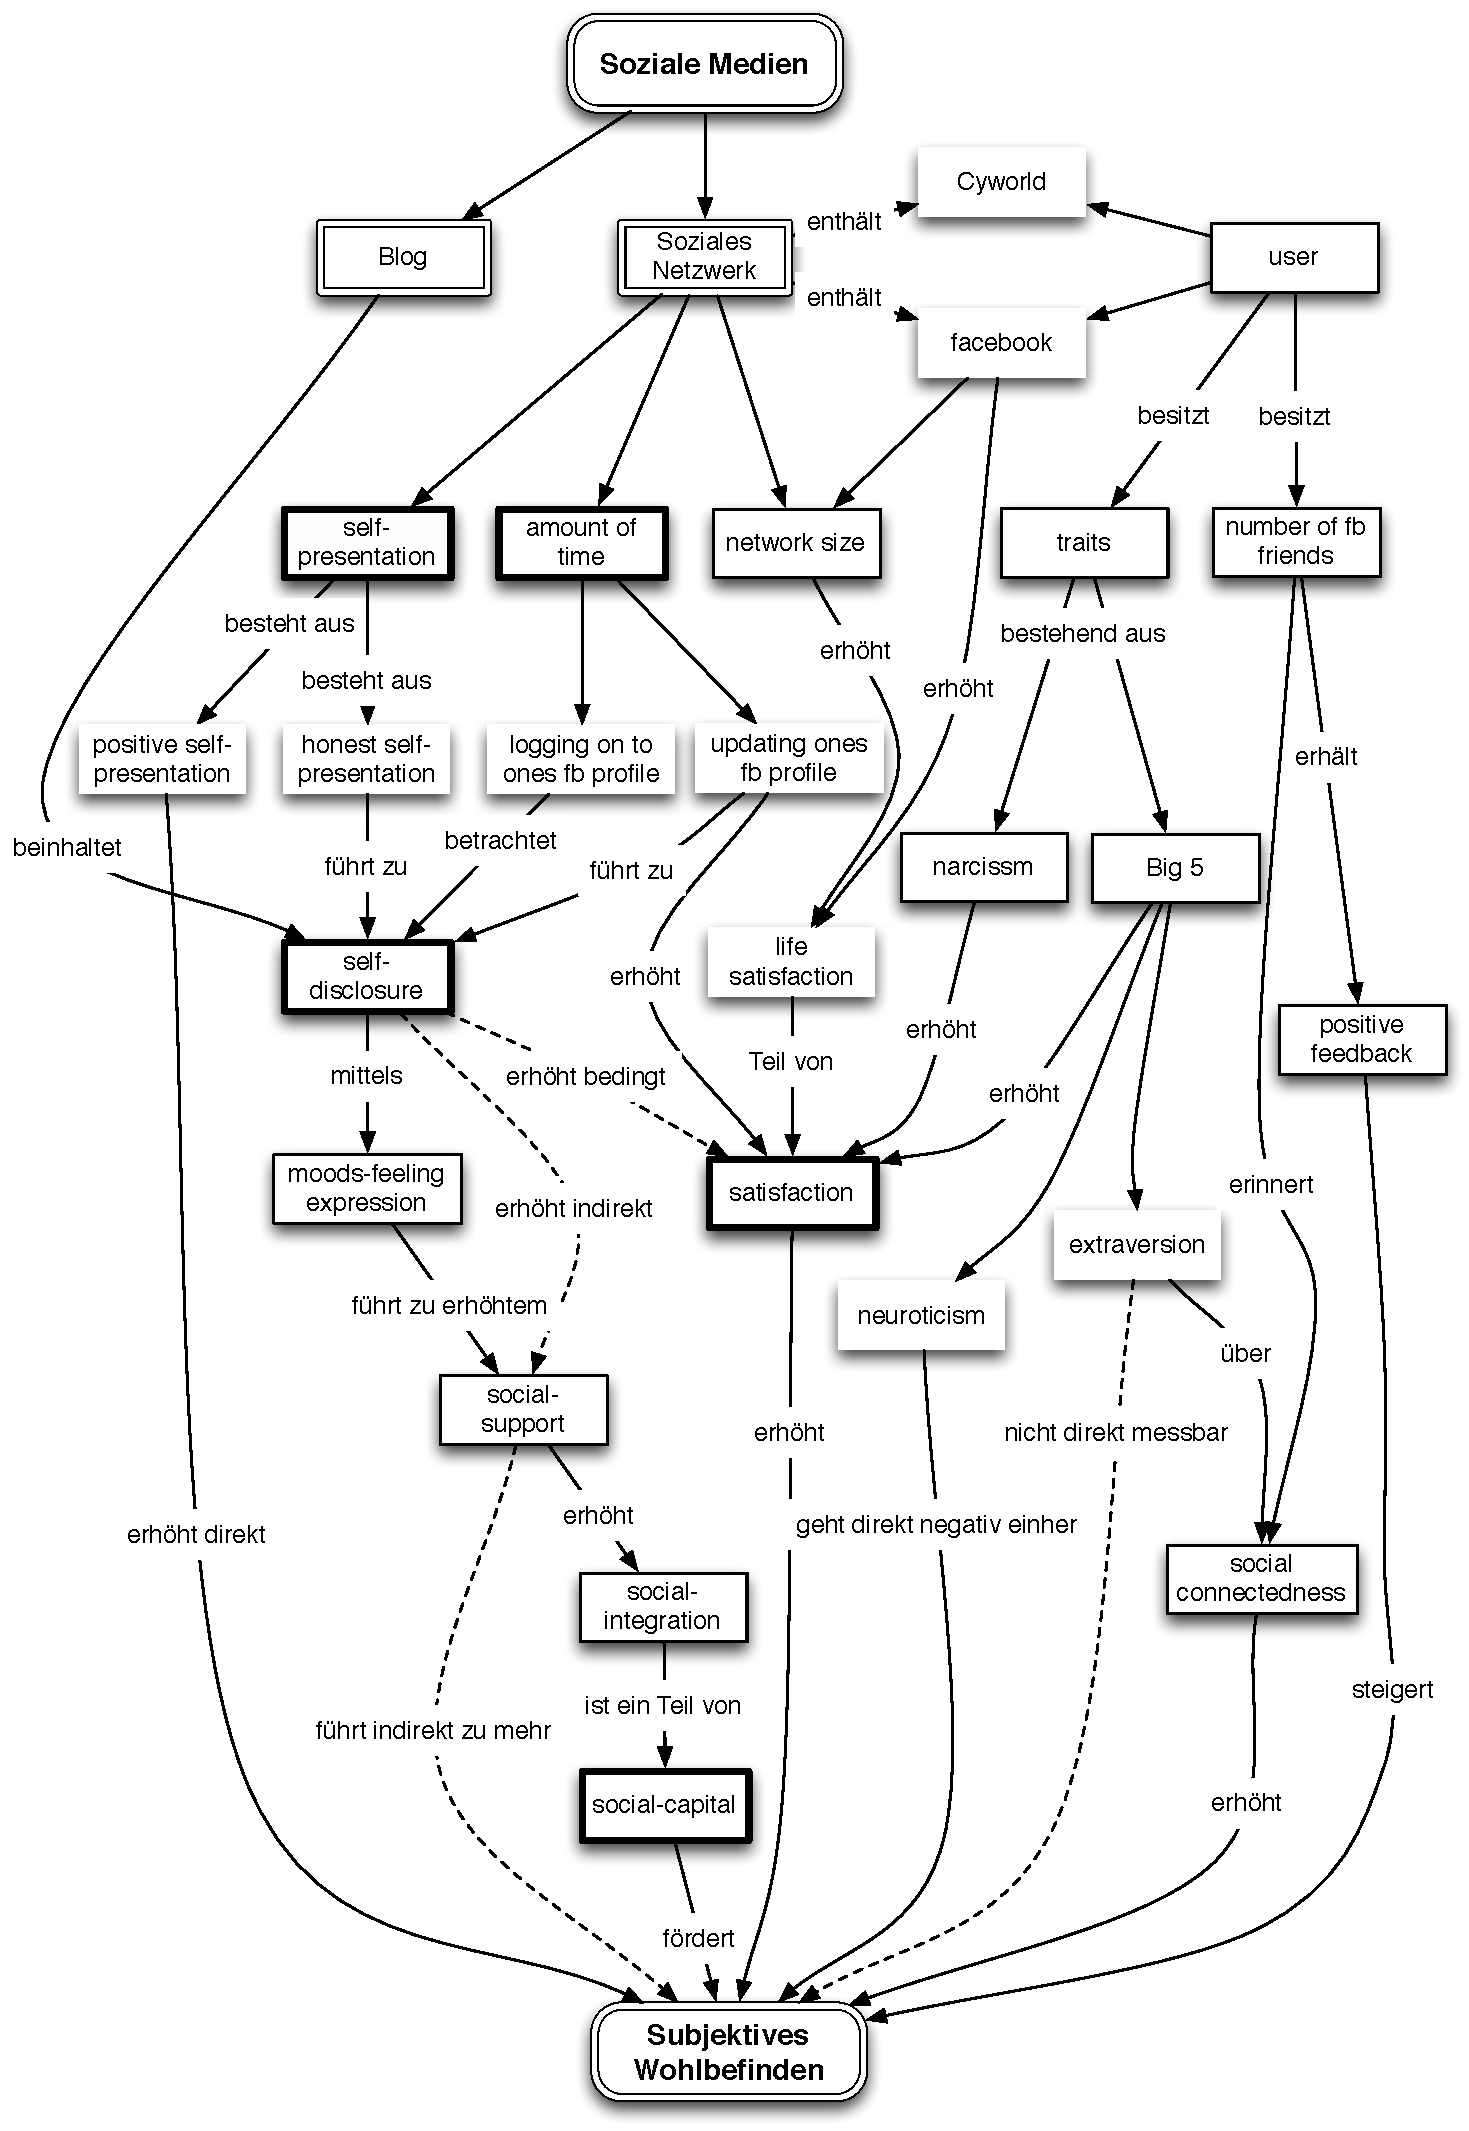
\includegraphics[width=0.8\textwidth]{images/grafiken/conceptMap_Swb_Sm_v2.pdf}
	\caption{ConceptMap - Subjektives Wohlbefinden und Soziale Medien}
	\label{fig.ConceptMapSwbSm}
\end{figure}

%UK Self-Presentation, Self-dicslosure und social capital
%----------------------------------------------------------------------
\section{\textit{Self-presentation}, \textit{self-disclosure} und \textit{social capital}}\label{sub.selfp}
In diesem Kapitel wird auf den Einfluss von \textit{self-presentation} und \textit{self-disclosure}, als Haupteinflussgrössen auf das \textit{\gls{swb}} eingegangen. \newline
%SubSec Einführung
\subsection{Einführung}\label{subsec.selfpEinführung}
Unter \textbf{self-presentation} (\textit{dt. Selbstdarstellung}) wird eine Strategie verstanden, die im Kontext von \textit{Facebook} näher untersucht wurde \cite[S.359ff]{Kim:2011}. \textit{Facebook} stellt nicht nur Mechanismen zur Verfügung, um Benutzerverbindungen untereinander grafisch darzustellen, sondern auch technologische Möglichkeiten wie sich Benutzer selber darstellen können \cite{Ellison:2007.1}. Je nach dem welche Möglichkeiten ein Benutzer verwendet (z.B.: Statusaktualisierung, erstellen und pflegen eines Fotoalbums, Nachrichten auf dem eigenen Profil posten, etc.) stellen sich diese Benutzer unterschiedlich getreu dar. In der Literatur wird innerhalb der \textit{\gls{cmc} (dt. Computervermittelte Kommunikation)} \cite{Tidwell:2002} und \textit{self-presentation} auf online Partnervermittlungsplattformen \cite{Gibbs:2006} zwischen zwei unterschiedlichen Strategien unterschieden: \textit{Positiver} und \textit{ehrlicher Selbstdarstellung}. Auf der einen Seite wird eine hohe ersichtliche Aktivität eines Benutzers auf \textit{Facebook} ihn dazu bewegen, sich möglichst positiv darzustellen \cite{Kimmerle:2008} und auf der anderen Seite werden sich Benutzer, die eine langfristige Beziehung anstreben, sich eher auf eine ehrliche Art präsentieren \cite{Gibbs:2006}. Die Frage stellt sich, ob eine positive und ehrliche Darstellung der eigenen Person auf \textit{Facebook} einen Einfluss auf das \gls{swb} hat.\newline
Im Gegensatz zur Darstellung eines Individuums, wie es auf \textit{Facebook} erfolgt, werden auf einem Journal \textit{(Blog)} Texte veröffentlicht. Ein persönliches Journal widerspiegelt die innere Welt eines Autors, was unter dem Begriff \textbf{self-disclosure} (\textit{dt. Selbstoffenbahrung}) verstanden wird. Ein Prozess, bei dem ein Individuum sein Gefühle, Gedanken, Erlebnisse und Informationen mit anderen Personen teilt \cite{Derlega:1993}. Baker und Moore gehen davon aus \cite{Baker:2008}, dass \textit{self-disclosure} dazu beitragen kann, existierende Beziehungen aufrecht zu erhalten und das eigene Beziehungsnetzwerk auszubauen. Beide Vorgänge werden gemäss Putnam \cite{Putnam:2000} als wichtige Faktoren für das \textit{soziale Kapital} oder \textbf{social capital} benötigt, welches erheblich zur Erhöhung des \gls{swb} beisteuert \cite{Sirgy:2006}.
%SubSec Ergebnisse
\subsection{Ergebnisse}\label{subsec.selfpErgebnisse}
Gemäss den Untersuchungen von \citeA[S.362]{Kim:2011} hat \textit{positive self-presentation} einen direkten positiven Effekt auf das \gls{swb}. Sie stellten fest, dass \textit{Facebook}-Benutzer glücklicher sind, wenn sie ihr Selbstbild durch eine positive Selbstdarstellung bekräftigen und unterstützen. Dieses Ergebnis wird durch die \textit{positive illusion theorie} von Taylor zusätzlich gestützt \cite{Taylor:1996,Taylor:1988}. Diese Theorie besagt, dass eine voreingenommene Erkenntnis über das Ich oder eine Erkenntnis, die durch eine Erhöhung des eigenen Ansehens entstanden ist, helfen kann mit stressvollen oder bedrohlichen Situationen besser umzugehen und sich dadurch glücklicher zu fühlen \textit{(feel happy)}. \newline
Im Gegenzug wirkte sich \textit{honest self-presentation} bei \citeA[S.362]{Kim:2011} indirekt positiv auf das \textit{\gls{swb}} aus, in dem die soziale Unterstützung aus dem Umfeld erhöht wahrgenommen wird. Dieses Ergebnis unterstreicht die Wichtigkeit von \textit{self-disclosure}, welches das Schlüsselement bei der Entwicklung von sozialen Online-Beziehungen darstellt \cite{Joinsen:2001}. \textit{Facebook}-Freunde sind eher gewillt ihresgleichen zu helfen, wenn diese Person das Bedürfnis über angemessene Selbstoffenbahrung kommuniziert und sich durch eine ehrliche Selbstdarstellung auf \textit{Facebook} präsentiert. Diese Unterstützung durch das soziale Umfeld \textit{(aus dem engl. social-support)} führt zu einem förderlichen \gls{swb} \cite{Greene:2006}.\newline
Eine weitere Studie von \citeA{Ko:2009} belegt, dass sich das Benehmen von Blogger durch \textit{self-disclosure} signifikant und direkt auf die soziale Integration und dadurch auf das soziale Kapital auswirkt, welches wiederum das \gls{swb} der Blogger erhöht. Gestützt wird dies dadurch, dass in den meisten publizierten Artikeln die Launen und Gefühle der Blogger eine entscheidende Rolle spielen. 93\% der Blogger geben an, dass der Ausdruck von Stress, Hemmungen, Druck und Verstimmungen in ihren Artikeln ausgedrückt werden. Diese Angaben decken sich mit den Resultaten von \citeA{Pennebaker:1997} die besagen, dass wenn Menschen ihre Gedanken zu ihren Launen und Gefühlen \textit{(engl. moods-feeling expression)} mit anderen Menschen durch Schreiben mitteilen, dies zu einer grösseren Unterstützung durch das soziale Umfeld \textit{(engl. social support)} und demzufolge zu einer höheren sozialen Integration \textit{(engl. social integration)} führt. Die soziale Integration wiederum ist ein Teil des sozialen Kapitals, welches eine Erhöhung des \gls{swb} voraussagt \cite{Ko:2009}.\newline
Zusammenfassend geht hervor, dass sowohl bei \citeA{Kim:2011} als auch bei \citeA{Ko:2009} der Einfluss von \gls{sm} mittels \textit{self-presentation, self-disclosure} und \textit{social-capital} einen positiven Einfluss auf das \gls{swb} haben.

%SubSec Diskussion
\subsection{Diskussion}\label{subsec.selfpDiskussion}
In den verwendeten Studien gemäss \citeA{Kim:2011} wurde die Messung des \gls{swb} mittels Selbsteinschätzung erstellt. Obwohl es sich dabei um eine verbreitete und adäquate Methode handelt \cite{Diener:2005}, ist sie nicht vor Fehler und Verzerrungen gefeit, die aufgrund der Antworten entstehen können (z.B.: soziale Erwünschtheit) siehe dazu \citeA{Diener:1991}. Antworten mit einer erhöhten \textit{Sozialen Erwünschtheit} könnten von Personen stammen, die sich gerne selber positiv darstellen, was zu einem positiven Zusammenhang zwischen \textit{positive self-presentation} und \gls{swb} führen könnte \cite{Diener:1991}.\newline
In der Studie von \citeA{Kim:2011} wurde vor allem Stichproben von \textit{Facebook}-Benutzern im Hochschulalter verwendet. Da sich die Nutzung auf die gesamte Öffentlichkeit erstreckt, sollte das Verhalten anhand der restlichen Benutzer untersucht werden (ausserhalb des Hochschulalters).

%UK Summe der verwendeten Zeit (amount of time)
%----------------------------------------------------------------------
\section{Summe der verwendeten Zeit \textit{(amount of time)}}\label{sub.amount}

%SubSec Einführung
\subsection{Einführung}\label{subsec.amountEinführung}

%SubSec Ergebnisse
\subsection{Ergebnisse}\label{subsec.amontErgebnisse}

%SubSec Diskussion
\subsection{Diskussion}\label{subsec.amountDiskussion}


%UK Benutzer Traits
%----------------------------------------------------------------------
\section{Benutzer Traits}\label{sub.traits}

%SubSec Einführung
\subsection{Einführung}\label{subsec.traitsEinführung}

%SubSec Ergebnisse
\subsection{Ergebnisse}\label{subsec.traitsErgebnisse}

%SubSec Diskussion
\subsection{Diskussion}\label{subsec.traitsDiskussion}


%UK Anzahl Facebook Freunde
%----------------------------------------------------------------------
\section{Anzahl \textit{Facebook} Freunde}\label{sub.friends}

%SubSec Einführung
\subsection{Einführung}\label{subsec.friendsEinführung}

%SubSec Ergebnisse
\subsection{Ergebnisse}\label{subsec.friendsErgebnisse}

%SubSec Diskussion
\subsection{Diskussion}\label{subsec.friendsDiskussion}
